% !TeX root = RJwrapper.tex
\title{Variable Importance Plots: An Introduction to the \pkg{vip} Package}
\author{by Brandon M. Greenwell and Bradley C. Boehmke}

\maketitle

\abstract{
In the era of “big data”, it is becoming more of a challenge to not only build state-of-the-art predictive models, but also gain an understanding of what’s really going on in the data. For example, it is often of interest to know which, if any, of the predictors in a fitted model are relatively influential on the predicted outcome. Some modern algorithms—like random forests and gradient boosted decision trees—have a natural way of quantifying the importance or relative influence of each feature. Other algorithms—like naive Bayes classifiers and support vector machines—are not capable of doing so and model-agnostic approaches are generally used to measure each predictor’s importance. Enter \pkg{vip}, an R package for constructing variable importance scores/plots for many types of supervised learning algorithms using model-based and novel model-agnostic approaches. We'll also discuss a novel way to display both feature importance and feature effects together using sparklines.
}

\strong{TODO:}

\begin{itemize}

  \item Discuss layout of the package (e.g., \code{vi()} vs. \code{vip()} and workhorse functions like \code{vi\_permute()}.
  \item Discuss strengths/weaknesses of different approaches.
  \item Discuss other packages (like \pkg{DALEX} and \pkg{iml}.
  \item DIscuss how PDP and ICE curve info is stored as an attribute whenever \code{method = "pdp"} or \code{method = "ice"}, respectively.
  \item Should we discuss interaction detection? Probably...(the $H$-statistic example, if correct, is motivation enough).
  \item Need a good motivating example (e.g., airfoil example from arXiv paper using the \pkg{SuperLearner} package).
  \item Better discussion of function arguments, especially for permutation approach.
  \item Parallel examples for PDP-, ICE-, and permuataion-based approaches.

\end{itemize}

% ------------------------------------------------------------------------------
\section{Introduction}
% ------------------------------------------------------------------------------

Variable importance (VI).

For illustration, we use one of the regression problems described in \citet{multivariate-friedman-1991} and \citet{bagging-breiman-1996}. These data are available in the \CRANpkg{mlbench package} \citep{mlbench-pkg}. The inputs consist of 10 independent variables uniformly distributed on the interval $\left[0,1\right]$; however, only 5 out of these 10 are actually used in the true model. Outputs are created according to the formula described in \code{?mlbench::mlbench.friedman1}. The code chunk below simulates 500 observations from the model default standard deviation.

\begin{example}
# Simulate training data
set.seed(101)  # for reproducibility
trn <- as.data.frame(mlbench::mlbench.friedman1(500))  # ?mlbench.friedman1

# Inspect data
tibble::as_tibble(trn)
#> Warning: `as.tibble()` is deprecated, use `as_tibble()` (but mind the new semantics).
#> This warning is displayed once per session.
#> # A tibble: 500 x 11
#>       x.1   x.2   x.3   x.4    x.5     x.6   x.7   x.8   x.9  x.10     y
#>     <dbl> <dbl> <dbl> <dbl>  <dbl>   <dbl> <dbl> <dbl> <dbl> <dbl> <dbl>
#>  1 0.372  0.406 0.102 0.322 0.693  0.758   0.518 0.530 0.878 0.763 14.9 
#>  2 0.0438 0.602 0.602 0.999 0.776  0.533   0.509 0.487 0.118 0.176 15.3 
#>  3 0.710  0.362 0.254 0.548 0.0180 0.765   0.715 0.844 0.334 0.118 15.1 
#>  4 0.658  0.291 0.542 0.327 0.230  0.301   0.177 0.346 0.474 0.283 10.7 
#>  5 0.250  0.794 0.383 0.947 0.462  0.00487 0.270 0.114 0.489 0.311 17.6 
#>  6 0.300  0.701 0.992 0.386 0.666  0.198   0.924 0.775 0.736 0.974 18.3 
#>  7 0.585  0.365 0.283 0.488 0.845  0.466   0.715 0.202 0.905 0.640 14.6 
#>  8 0.333  0.552 0.858 0.509 0.697  0.388   0.260 0.355 0.517 0.165 17.0 
#>  9 0.622  0.118 0.490 0.390 0.468  0.360   0.572 0.891 0.682 0.717  8.54
#> 10 0.546  0.150 0.476 0.706 0.829  0.373   0.192 0.873 0.456 0.694 15.0 
#> # … with 490 more rows
\end{example}


% ------------------------------------------------------------------------------
\section{Model-specific VI}
% ------------------------------------------------------------------------------

Some machine learning algorithms have their own way of quantifying variable Importance. We describe some of these in the subsection that follow. The issue with model-specific VI scores is that they are not necessarily comparable across different types of models. For example, directly computing the impurity-based VI scores from tree-based models to the 𝑡-statistic from linear models.

\subsection{Trees and tree ensembles}

Decision trees probably offer the most natural model-based approach to quantifying the importance of each feature. In a binary decision tree, at each node 𝑡, a single predictor is used to partition the data into two homogeneous groups. The chosen predictor is the one that maximizes some measure of improvement 𝑖ˆ𝑡. The relative importance of predictor 𝑥 is the sum of the squared improvements over all internal nodes of the tree for which 𝑥 was chosen as the partitioning variable; see Breiman, Friedman, and Charles J. Stone (1984) for details. This idea also extends to ensembles of decision trees, such as RFs and GBMs. In ensembles, the improvement score for each predictor is averaged across all the trees in the ensemble. Fortunately, due to the stabilizing effect of averaging, the improvement-based VI metric is often more reliable in large ensembles (see Hastie, Tibshirani, and Friedman 2009, pg. 368). RFs offer an additional method for computing VI scores. The idea is to use the leftover out-of-bag (OOB) data to construct validation-set errors for each tree. Then, each predictor is randomly shuffled in the OOB data and the error is computed again. The idea is that if variable 𝑥 is important, then the validation error will go up when 𝑥 is perturbed in the OOB data. The difference in the two errors is recorded for the OOB data then averaged across all trees in the forest.

To illustrate, we fit a CART-like regression tree, RF, and GBM to the simulated training data. (Note: there are a number of different packages available for fitting these types of models, we just picked popular and efficient implementations for illustration.)

\begin{example}
# Load required packages
library(rpart)          # for fitting CART-like decision trees
library(randomForest)   # for fitting random forests
library(xgboost)        # for fitting GBMs

# Fit a single regression tree
tree <- rpart(y ~ ., data = trn)

# Fit a random forest
set.seed(101)
rfo <- randomForest(y ~ ., data = trn, importance = TRUE)

# Fit a GBM
set.seed(102)
bst <- xgboost(
  data = data.matrix(subset(trn, select = -y)),
  label = trn$y, 
  objective = "reg:linear",
  nrounds = 100, 
  max_depth = 5, 
  eta = 0.3,
  verbose = 0  # suppress printing
)
\end{example}

Each of the above packages include the ability to compute VI scores for all the features in the model; however, the implementation is rather package specific, as shown in the code chunk below. The results are displayed in Figure~\ref{fig:vi-plots}.

\begin{example}
# Extract VI scores from each model
vi_tree <- tree$variable.importance
vi_rfo <- rfo$variable.importance
vi_bst <- xgb.importance(model = bst)
\end{example}

\begin{figure}[!htb]
  \centering 
  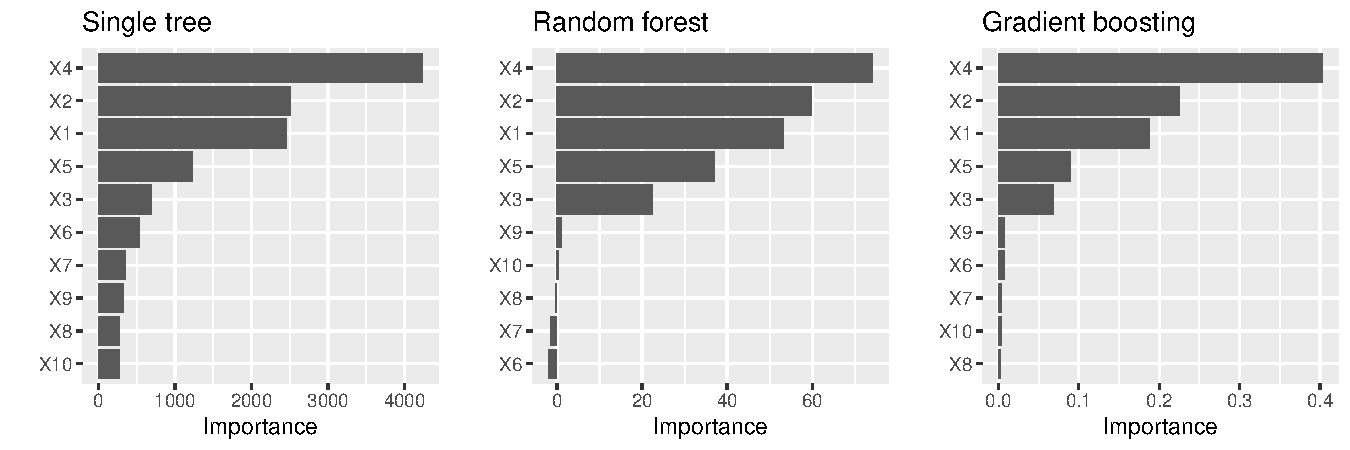
\includegraphics[width=1\linewidth]{figures/vi-plots} 
  \caption{Model-based VIPs for the three different tree-based models.}
  \label{fig:vi-plots}
\end{figure}

As we would expect, all three methods rank the variables \code{x.1}--\code{x.5} as more important than the others. While this is good news, it is unfortunate that we have to remember the different functions and ways of extracting and plotting VI scores from various model fitting functions. This is where \CRANpkg{vip} \citep{vip-pkg} can help...one function to rule them all! Once \pkg{vip} is loaded, we can use \code{vi()} to extract a tibble of VI scores.

\begin{example}
library(vip)

vi(tree)  # CART-like decision tree
#> # A tibble: 10 x 2
#>    Variable Importance
#>    <chr>         <dbl>
#>  1 x.4           4234.
#>  2 x.2           2513.
#>  3 x.1           2461.
#>  4 x.5           1230.
#>  5 x.3            688.
#>  6 x.6            533.
#>  7 x.7            357.
#>  8 x.9            331.
#>  9 x.8            276.
#> 10 x.10           275.

vi(rfo)   # RF
#> # A tibble: 10 x 2
#>    Variable Importance
#>    <chr>         <dbl>
#>  1 x.4          74.2  
#>  2 x.2          59.9  
#>  3 x.1          53.3  
#>  4 x.5          37.1  
#>  5 x.3          22.5  
#>  6 x.9           1.05 
#>  7 x.10          0.254
#>  8 x.8          -0.408
#>  9 x.7          -1.56 
#> 10 x.6          -2.00

vi(bst)   # GBM
#> # A tibble: 10 x 2
#>    Variable Importance
#>    <chr>         <dbl>
#>  1 x.4         0.403  
#>  2 x.2         0.225  
#>  3 x.1         0.189  
#>  4 x.5         0.0894 
#>  5 x.3         0.0682 
#>  6 x.9         0.00802
#>  7 x.6         0.00746
#>  8 x.7         0.00400
#>  9 x.10        0.00377
#> 10 x.8         0.00262
\end{example}


Notice how the \code{vi()} function always returns a tibble with two columns: \code{Variable} and \code{Importance}. Also, by default, \code{vi()} always orders the VI scores from highest to lowest; this, among other options, can be controlled by the user (see \code{?vip::vi} for details). Plotting VI scores with \code{vip()} is just as straightforward. For example, the following code can be used to reproduce Figure~\ref{fig:vi-plots}.

\begin{example}
p1 <- vip(tree) + ggtitle("Single tree")
p2 <- vip(rfo) + ggtitle("Random forest")
p3 <- vip(bst) + ggtitle("Gradient boosting")

# Figure 1
grid.arrange(p1, p2, p3, nrow = 1)
\end{example}

Notice how the \code{vip()} function always returns a \code{"ggplot"} object (by default, this will be a bar plot). For large models with many features, a dot plot is more effective (in fact, a number of useful plotting options can be fiddles with). Below we call \code{vip()} and change a few useful options (the resulting plot is displayed in Figure~\ref{fig:dot-plot}).

\begin{example}
# Load required packages
library(ggplot2)  # for theme_light() function

vip(bst, num_features = 5, bar = FALSE, color, horizontal = FALSE, 
    color = "red", shape = 17, size = 4) +
  theme_light()
\end{example}

\begin{figure}[!htb]
  \centering 
  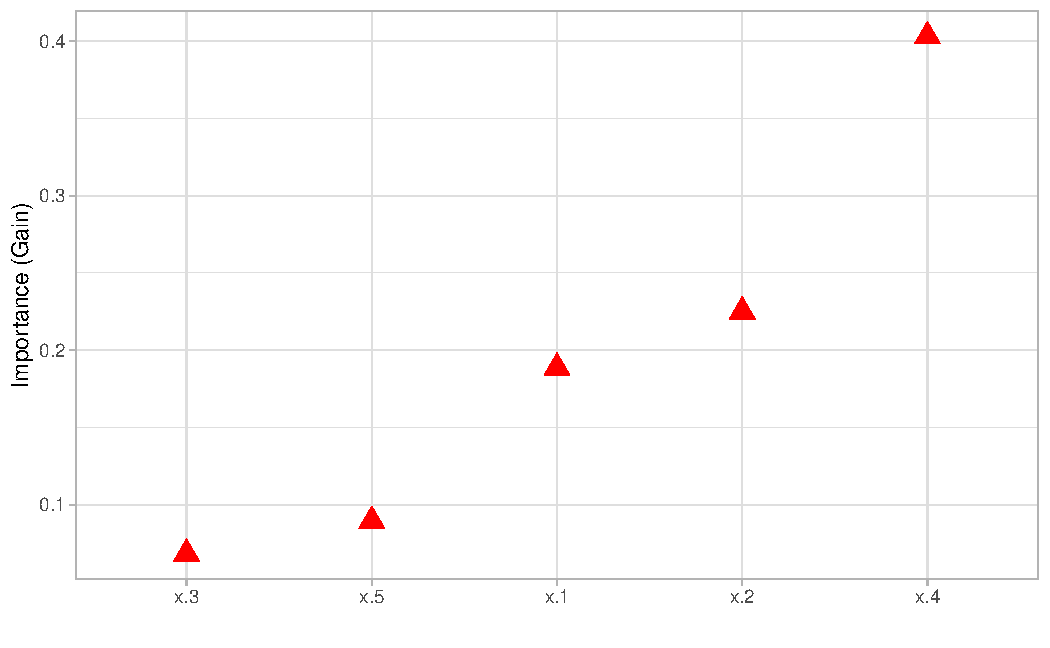
\includegraphics[width=1\linewidth]{figures/dot-plot} 
  \caption{Illustrating various options available in \code{vip()}.}
  \label{fig:dot-plot}
\end{figure}


\subsection{Linear models}

In multiple linear regression, or linear models (LMs), the absolute value of the $t$-statistic (or some other scaled variant of the estimated coefficients) is commonly used as a measure of VI. The same idea also extends to generalized linear models (GLMs). In the code chunk below, we fit an LM to the simulated \code{trn} data set allowing for all main and two-way interaction effects, then use the \code{step()} function to perform backward elimination. The resulting VIP is displayed in Figure~\ref{fig:vip-step}.

\begin{example}
# Fit a LM
linmod <- lm(y ~ .^2, data = trn)
backward <- step(linmod, direction = "backward", trace = 0)

# Extract VI scores
vi(backward)
#> # A tibble: 21 x 3
#>    Variable Importance Sign 
#>    <chr>         <dbl> <chr>
#>  1 x.4           14.2  POS  
#>  2 x.2            7.31 POS  
#>  3 x.1            5.63 POS  
#>  4 x.5            5.21 POS  
#>  5 x.3:x.5        2.46 POS  
#>  6 x.1:x.10       2.41 NEG  
#>  7 x.2:x.6        2.41 NEG  
#>  8 x.1:x.5        2.37 NEG  
#>  9 x.10           2.21 POS  
#> 10 x.3:x.4        2.01 NEG  
#> # … with 11 more rows

# Plot VI scores
vip(backward, num_features = length(coef(backward)), 
    bar = FALSE, horizontal = FALSE)
\end{example}

\begin{figure}[!htb]
  \centering 
  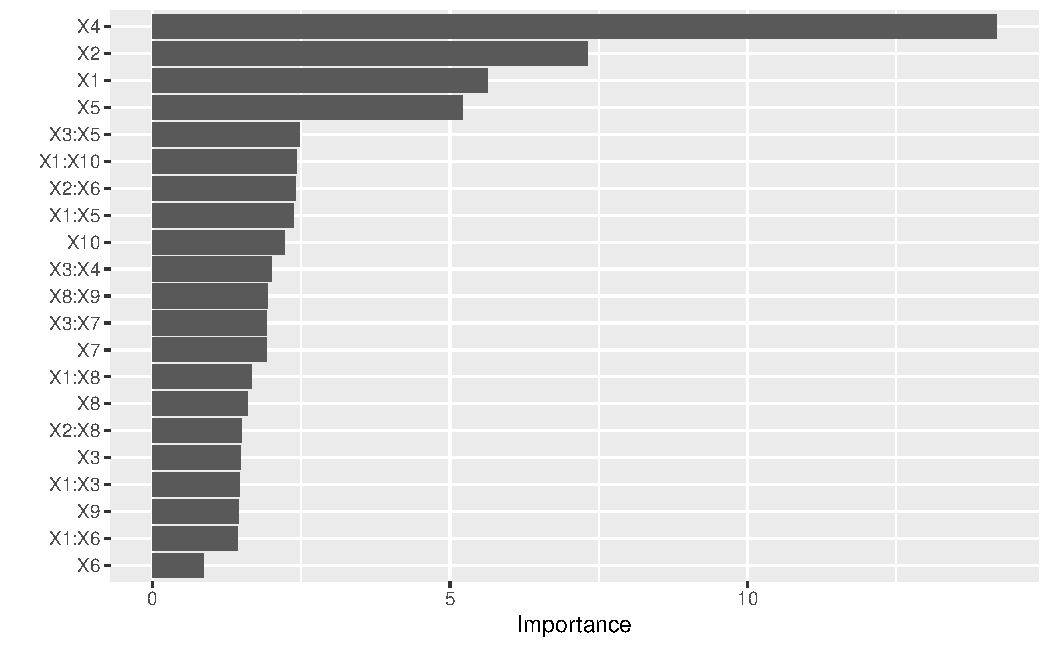
\includegraphics[width=1\linewidth]{figures/vip-step} 
  \caption{Example VIP from a linear model.}
  \label{fig:vip-step}
\end{figure}

One issue with computing VI scores for LMs using the $t$-statistic approach is that a score is assigned to each term in the model, rather than to just each feature! We can solve this problem using one of the model-agnostic approaches discussed later.

Multivariate adaptive regression splines (MARS), which were introduced in \citet{multivariate-friedman-1991}, is an automatic regression technique which can be seen as a generalization of multiple linear regression and generalized linear models. In the MARS algorithm, the contribution (or VI score) for each predictor is determined using a generalized cross-validation (GCV) statistic. An example using the \CRANpkg{earth} package \citep{earth-pkg} is given below (the results are plotted in Figure~\ref{fig:vip-earth}):

\begin{example}
# Load required packages
library(earth)

# Fit a MARS model
mars <- earth(y ~ ., data = trn, degree = 2, pmethod = "exhaustive")

# Extract VI scores
vi(mars)
#> # A tibble: 10 x 2
#>    Variable Importance
#>    <chr>         <dbl>
#>  1 x.4           100  
#>  2 x.1            83.2
#>  3 x.2            83.2
#>  4 x.5            59.3
#>  5 x.3            43.5
#>  6 x.6             0  
#>  7 x.7             0  
#>  8 x.8             0  
#>  9 x.9             0  
#> 10 x.10            0

# Plot VI scores
vip(mars)
\end{example}

\begin{figure}[!htb]
  \centering 
  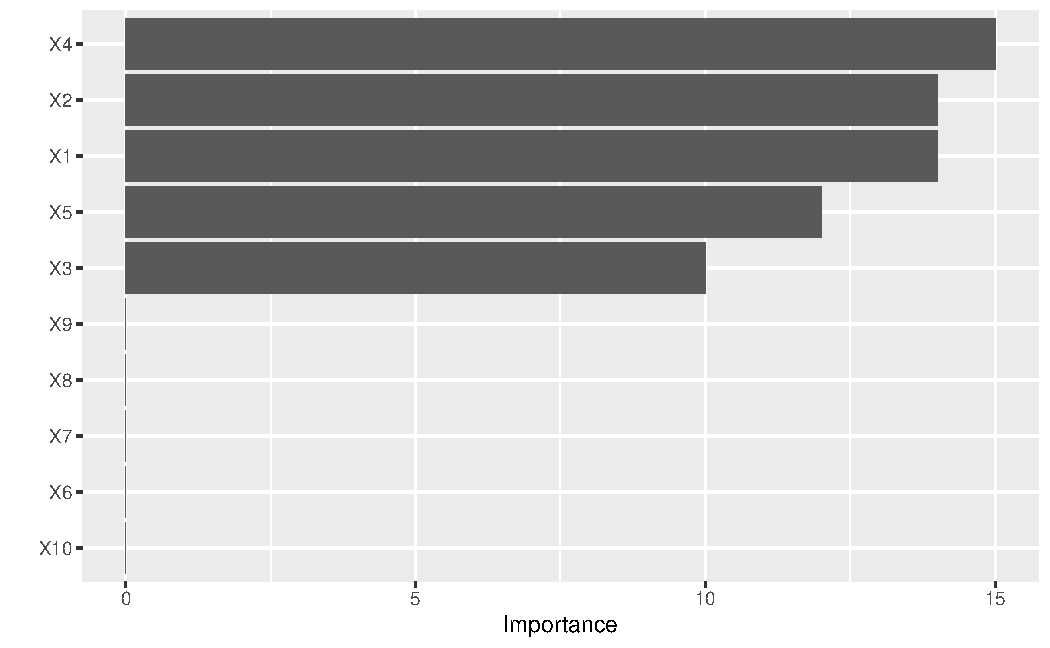
\includegraphics[width=1\linewidth]{figures/vip-earth} 
  \caption{Example VIP from a MARS model}.
  \label{fig:vip-earth}
\end{figure}

\subsection{Neural networks}

For neural netwroks (NNs), two popular methods for constructing VI scores are the Garson algorithm \citep{interpreting-garson-1991}, later modified by \citet{back-goh-1995}, and the Olden algorithm \citep{accurate-olden-2004}. For both algorithms, the basis of these importance scores is the network’s connection weights. The Garson algorithm determines VI by identifying all weighted connections between the nodes of interest. Olden’s algorithm, on the other hand, uses the product of the raw connection weights between each input and output neuron and sums the product across all hidden neurons. This has been shown to outperform the Garson method in various simulations. For DNNs, a similar method due to \citet{data-gedeon-1997} considers the weights connecting the input features to the first two hidden layers (for simplicity and speed); but this method can be slow for large networks. We illustrate these two methods below using \code{vip()} with the \CRANpkg{nnet} package \citep{nnet-pkg} (see the results in Figure~\ref{}).

\strong{FIXME: Add vip support for these two methods!}

\begin{example}
# Load required packages
library(nnet)

# Fit a neural network
set.seed(0803)
nn <- nnet(y ~ ., data = trn, size = 7, decay = 0.1, linout = TRUE)

# VIPs
p1 <- vip(nn, method = "garson")
p2 <- vip(nn, method = "olsen")

# Figure X
grid.arrange(p1, p2, nrow = 1)
\end{example}


% ------------------------------------------------------------------------------
\section{Model-agnostic VI}
% ------------------------------------------------------------------------------

Model-agnostic interpredibility separates interpretation from the model. Compared to model-specific approaches, model-agnostic VI methods are more flexible (since they can be applied to any supervised learning algorithm). In this section, we discuss model-agnostic methods for quantifying global feature importance using three different approaches: 1) \dfn{partial dependence plots} (PDPs), 2) \dfn{individual conditional expectation} (ICE) curves, and 3) permutation-based feature importance. For details on approaches 1)--2), see \citet{greenwell-simple-2018}.

Our first model-agnostic approach is based on quantifying the "flatness" of the PDPs of each feature. PDPs help visualize the effect of low cardinality subsets of the feature space on the estimated prediction surface (e.g., main effects and two/three-way interaction effects.). PDPs provide model-agnostic interpretations and can be constructed in the same way for any supervised learning algorithm; for an overview, see \citet{greenwell-pdp-2017}. Below, we fit a projection pursuit regression (PPR) model and construct PDPs for each feature using the \CRANpkg{pdp} package \citet{greenwell-pdp-2017}. The results are displayed in Figure~\ref{fig:pdp-ppr}. Notice how the PDPs for the uninformative features are relatively flat compared to the PDPs for features \code{x.1}--\code{x.2}!

\begin{example}
# Load required packages
library(pdp)

# Fit a PPR model (nterms was chosen using the caret package with 5 repeats of 
# 5-fold cross-validation)
pp <- ppr(y ~ ., data = trn, nterms = 11)  

# PDPs for all 10 features
features <- paste0("x.", 1:10)
pdps <- lapply(features, FUN = function(feature) {
  pd <- partial(pp, pred.var = feature)
  autoplot(pd) + 
    ylim(range(trn$y)) + 
    theme_light()
})
grid.arrange(grobs = pdps, ncol = 5)
\end{example}

\begin{figure}[!htb]
  \centering 
  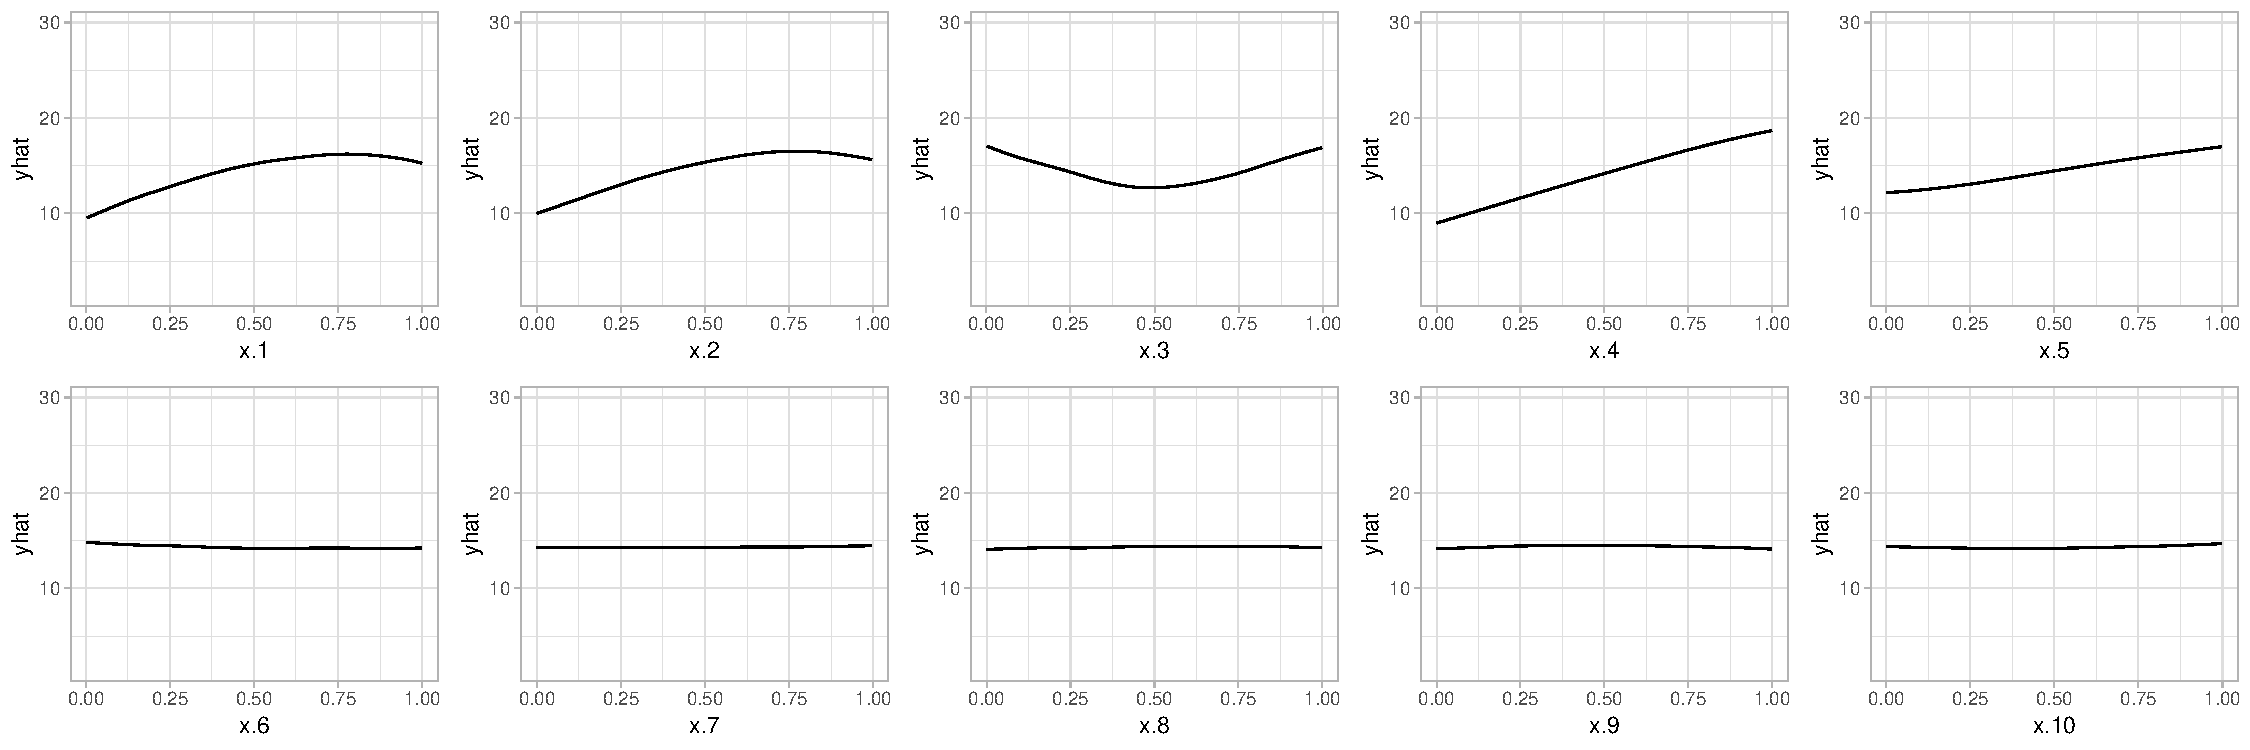
\includegraphics[width=1\linewidth]{figures/pdp-ppr} 
  \caption{PDPs of main effects in the PPR model.}
  \label{fig:pdp-ppr}
\end{figure}

Next, we compute PDP-based VI scores for the PPR and NN models. The PDP method constructs VI scores that quantify the "flatness" of each PDP (by default, this is defined by computing the standard deviation of the $y$-axis values for each PDP). To use the PDP method, specify \code{method = "pdp"} in the call to \code{vi()} or \code{vip()}:

\begin{example}
# Fit a PPR model (nterms was chosen using the caret package with 5 repeats of 
# 5-fold cross-validation)
pp <- ppr(y ~ ., data = trn, nterms = 11)  

# Plot VI scores
p1 <- vip(pp, method = "pdp") + ggtitle("PPR")
p2 <- vip(nn, method = "pdp") + ggtitle("NN")

# Figure X
grid.arrange(p1, p2, ncol = 2)
\end{example}

In Figure~\ref{fig:vip-pp-nn} we display the PDP-based feature improtance for the previously obtained PPR and NN models. These VI scores essentially capture the variability in the partial dependence values for each main effect.

\begin{figure}[!htb]
  \centering 
  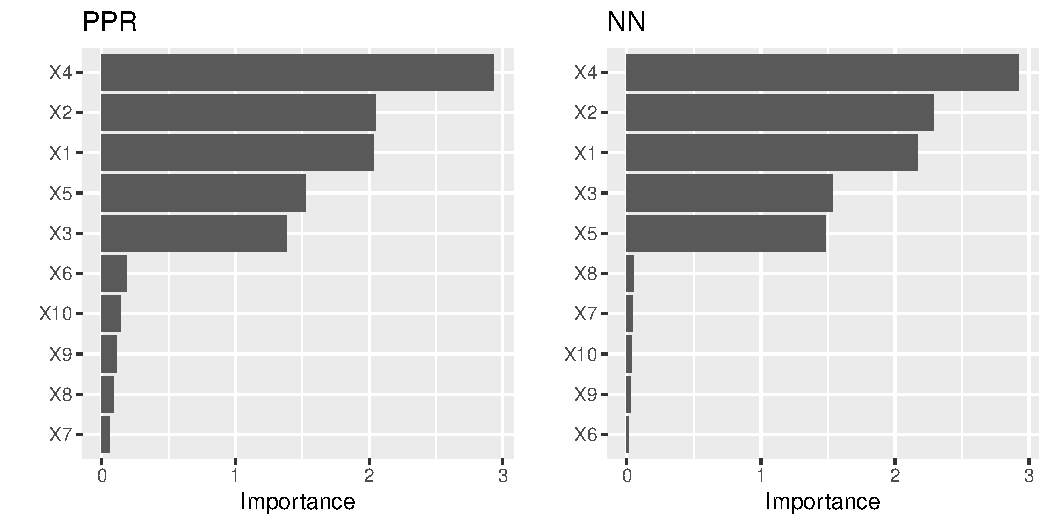
\includegraphics[width=1\linewidth]{figures/vip-ppr-nn} 
  \caption{PDP-based feature importance for the PPR and NN models.}
  \label{fig:pdp-ppr-nn}
\end{figure}

\subsection{ICE curve method}

The ICE curve method is similar to the PDP method. The only difference is that we measure the "flatness" of each ICE curve and then aggregate the results (e.g., by averaging). If there are no (substantial) interaction effects, using \code{method = "ice"} will produce results similar to using \code{method = "pdp"}. However, if strong interaction effects are present, they can obfuscate the main effects and render the PDP-based approach less useful (since the PDPs for important features can be relatively flat when certain interactions are present; see \citet{goldstein-peeking-2015} for details). In fact, it is probably safest to always use \code{method = "ice"}.

Below, we display the ICE curves for each feature in the PP model using the same $y$-axis scale; see Figure~\ref{fig:ice-ppr}. Again, there is a clear difference between the ICE curves for features \code{x.1}--\code{x.5} and \code{x.6}--\code{x.10}; the later being relatively flat by comparison. Also, notice how the ICE curves within each feature are relatively parallel (if the ICE curves within each feature were perfectly parallel, the standard deviation for each curve would be the same and the results will be identical to the PDP method). In this example, the interaction term between \code{x.1} and \code{x.2} does not obfuscate the PDPs for the main effects and the results are not much different.

\begin{example}
# ICE curves for all 10 features
ice_curves <- lapply(features, FUN = function(feature) {
  ice <- partial(pp, pred.var = feature, ice = TRUE)
  autoplot(ice, alpha = 0.1) + 
    ylim(range(trn$y)) +
    theme_light()
})

# Figure X
grid.arrange(grobs = ice_curves, ncol = 5)
\end{example}

\begin{figure}[!htb]
  \centering 
  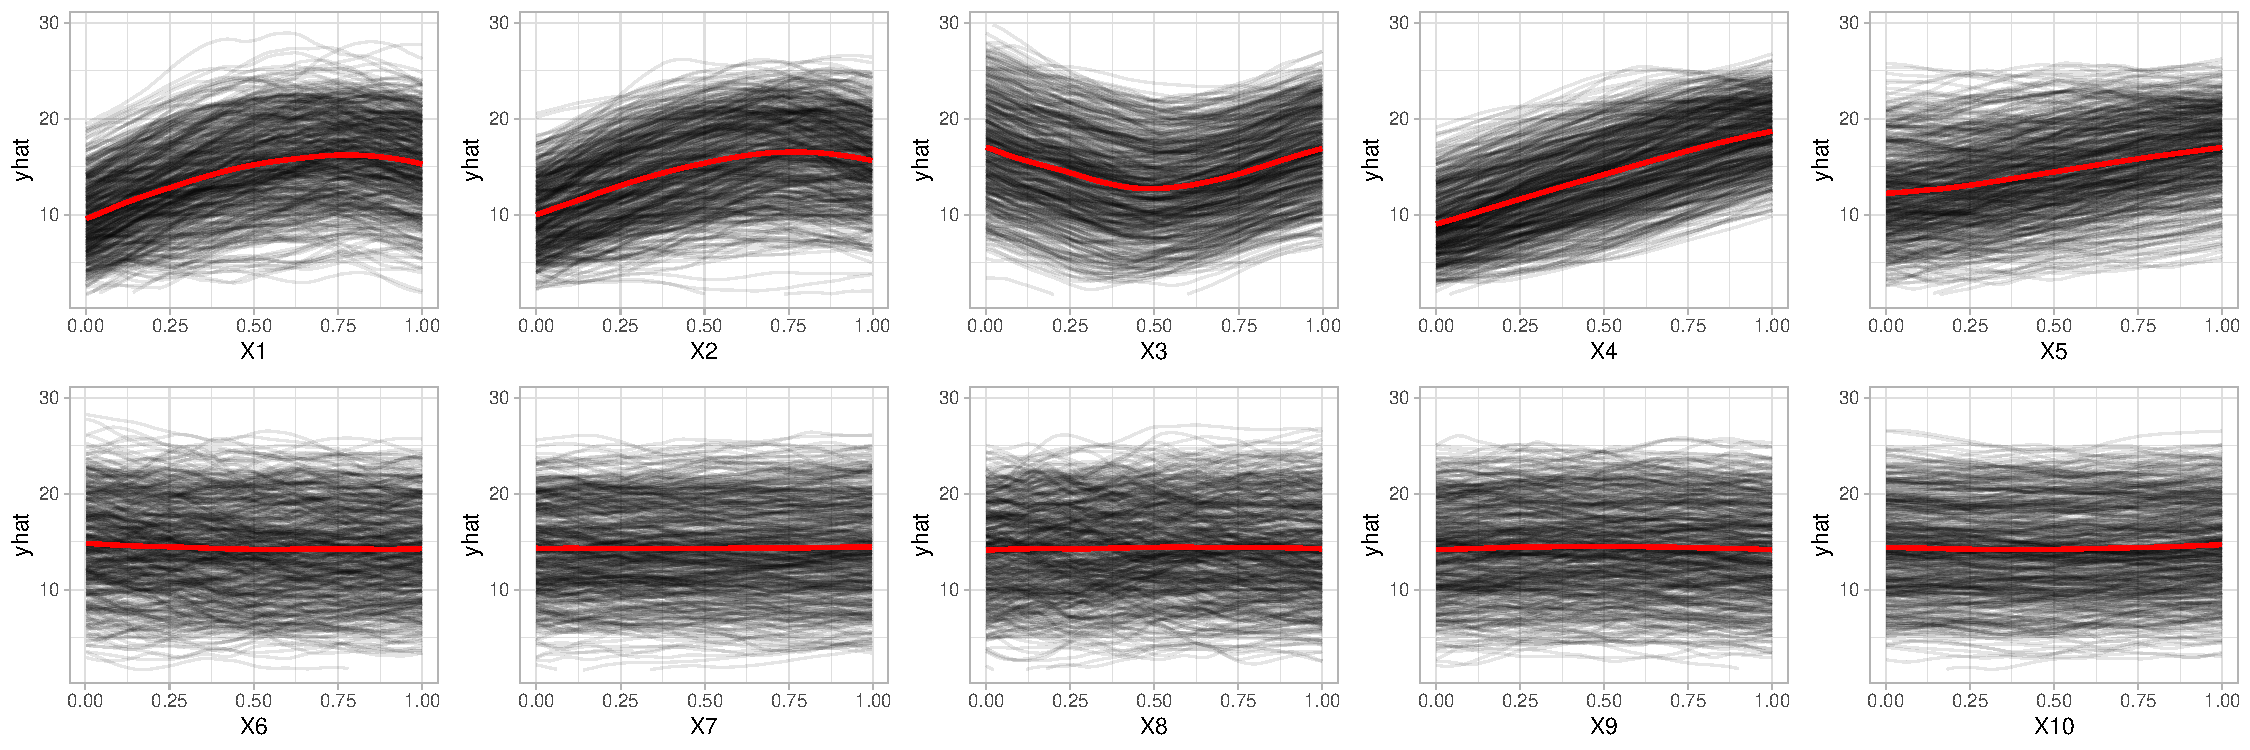
\includegraphics[width=1\linewidth]{figures/ice-ppr} 
  \caption{ICE curves for each feature in the PPR model. The red curve represents the PDP (i.e., the averaged ICE curves).}
  \label{fig:ice-ppr}
\end{figure}

Obtaining the ICE-based feature importance scores is also straightforward. The results in Figure~\ref{fig:vip-ice-ppr-nn} are similar to those obtained using the PDP method.

\begin{example}
# Plot VI scores
p1 <- vip(pp, method = "ice") + ggtitle("PPR")
p2 <- vip(nn, method = "ice") + ggtitle("NN")

# Figure X
grid.arrange(p1, p2, ncol = 2)
\end{example}

\begin{figure}[!htb]
  \centering 
  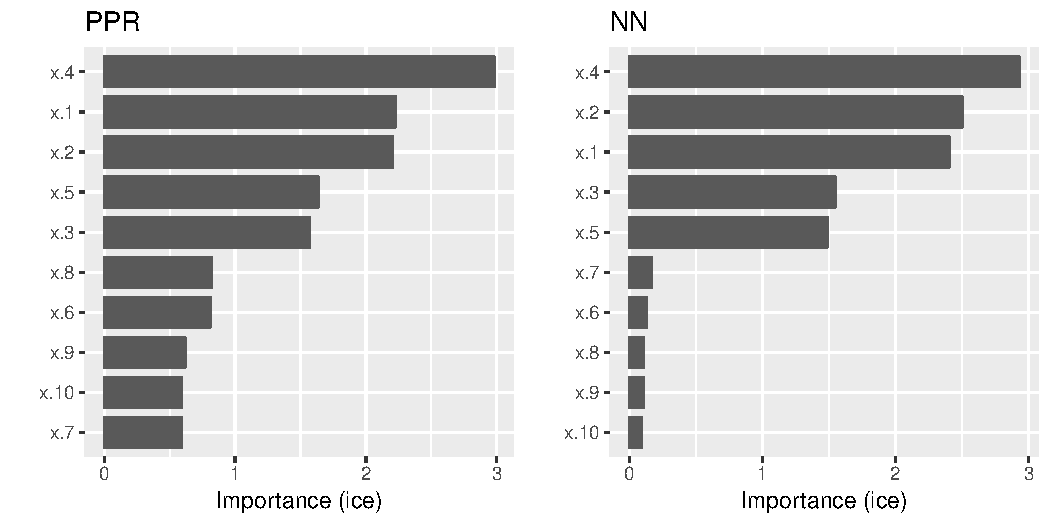
\includegraphics[width=1\linewidth]{figures/vip-ice-ppr-nn} 
  \caption{ICE-based feature importance for the PPR and NN models.}
  \label{fig:vip-ice-ppr-nn}
\end{figure}


\subsection{Permutation method}

The permutation method exists in various forms and was made popular in \citet{random-breiman-2001} for random forests. The permutation approach used in \pkg{vip} is quite simple. The idea is that if we randomly permute thse values of an important feature in the training data, the training performance would degrade (since permuting the values of a feature effectively destroys any relationship between that feature and the target variable). This of course assumes that the model has been properly tuned (e.g., using cross-validation) and is not over fitting. The permutation approach uses the difference between some baseline performance measure (e.g., training $R^2$, AUC, or RMSE) and the same performance measure obtained after permuting the values of a particular feature in the training data (\strong{Note:} the model is NOT refit to the training data after randomly permuting the values of a feature). To use the permutation approach, specify \code{method = "permute"} in the call to \code{vi()} or \code{vip()}. Note that using \code{method = "permute"} requires specifying a few additional arguments; see \code{?vi\_permute} for details.

An example is given below for the previously fitted PPR and NN models. The result, which are displayed in Figure~\ref{fig:vip-permute-ppr-nn}, agree with those obtained using the PDP- and ICE-based methods.

\begin{example}
# Plot VI scores
set.seed(2021)  # for reproducibility
p1 <- vip(pp, method = "permute", target = "y", metric = "rsquared",
          pred_fun = predict) + ggtitle("PPR")
p2 <- vip(nn, method = "permute", target = "y", metric = "rsquared",
          pred_fun = predict) + ggtitle("NN")

# Figure X
grid.arrange(p1, p2, ncol = 2)
\end{example}

\begin{figure}[!htb]
  \centering 
  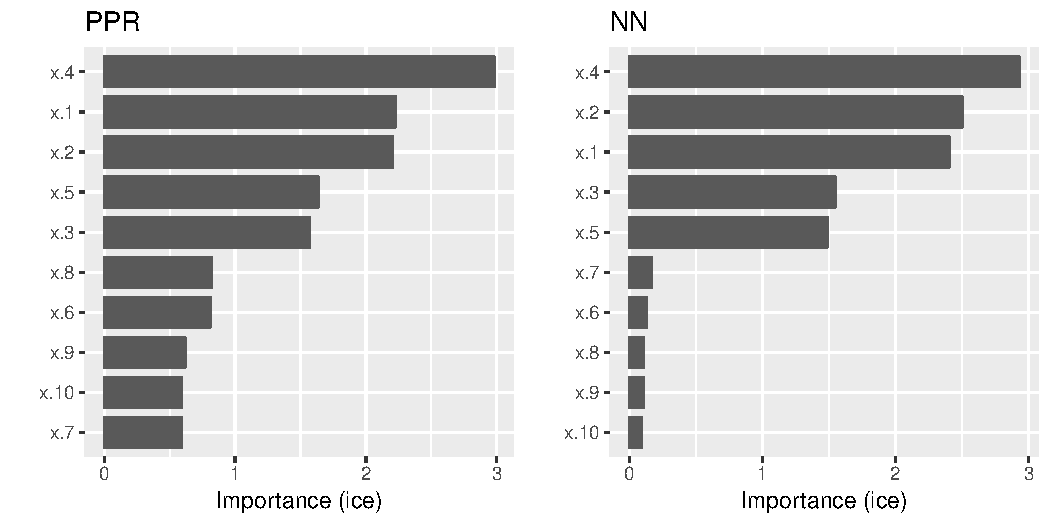
\includegraphics[width=1\linewidth]{figures/vip-ice-ppr-nn} 
  \caption{Permutation-based feature importance for the PPR and NN models.}
  \label{fig:vip-permute-ppr-nn}
\end{figure}

Tne permutation approach introduces randomness into the procedure and therefore should be run more than once if computationally feasible. Fortunately, this also allows us to compute standard errors for the estimated feature importance, as illustaretd in the example below where we specify `nsim = 10` to request that each feature be permuted 10 times and the results averaged together.

\begin{example}
# A tibble: 10 x 3
#>    Variable Importance   StDev
#>    <chr>         <dbl>   <dbl>
#>  1 x.4          0.586  0.0188 
#>  2 x.2          0.416  0.0184 
#>  3 x.1          0.377  0.0162 
#>  4 x.5          0.222  0.0155 
#>  5 x.3          0.183  0.00936
#>  6 x.6          0.0620 0.00379
#>  7 x.8          0.0603 0.00378
#>  8 x.9          0.0389 0.00417
#>  9 x.7          0.0373 0.00321
#> 10 x.10         0.0348 0.00290
\end{example}


% ------------------------------------------------------------------------------
\section{Use sparklines to characterize feature effects}
% ------------------------------------------------------------------------------

Starting with \pkg{vip} 0.1.3, we have included a new function \code{vit()} for constructing HTML-based feature importance tables. The primary difference between \code{vi()} and \code{vit()} is that the latter includes an \code{Effect} column that displays a sparkline representation of the partial dependence function for each feature. This is a concise way to display both feature importance and feature effect information in a single table. See \code{?vip::vit} for details. We illustrate the basic use of \code{vit()} in the code chunks below.

\begin{example}
# First, compute a tibble of variable importance scores using any method
var_imp <- vi(rfo, method = "permute", metric = "rmse", target = "y")

# Next, convert to an html-based data table with sparklines
vit(var_imp, fit = rfo)
\end{example}

\begin{figure}[!htb]
  \centering 
  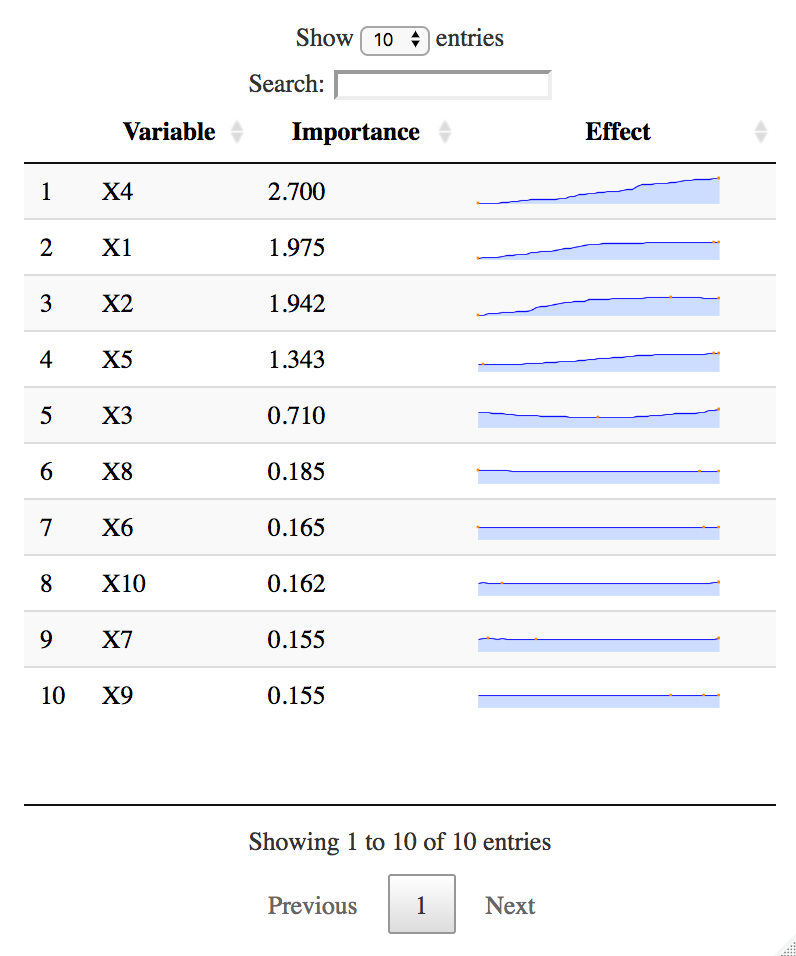
\includegraphics[width=1\linewidth]{figures/sparklines} 
  \caption{VIP with sparkline representation of feature effects.}
  \label{fig:sparklines}
\end{figure}


% ------------------------------------------------------------------------------
\section{Ames housing example}
% ------------------------------------------------------------------------------

TBD.


% ------------------------------------------------------------------------------
\section{Summary}
% ------------------------------------------------------------------------------

TBD.


\bibliography{pkg-vip}

\address{Brandon M. Greenwell\\
  Department of Mathematics and Statistics\\
  Wright State University\\
  3640 Colonel Glenn Hwy\\ 
  Dayton, OH 45435\\
  United States of America\\
  ORCiD: \href{https://orcid.org/0000-0002-8120-0084}{0000-0002-8120-0084}\\
  \email{greenwell.brandon@gmail.com}}

\address{Bradley C. Boehmke\\
  University of Cincinnati\\
  2925 Campus Green Dr\\
  Cincinnati, OH 45221\\
  United States of America\\
  ORCiD: \href{https://orcid.org/0000-0002-3611-8516}{0000-0002-3611-8516}\\
  \email{bradleyboehmke@gmail.com}}
